\documentclass{article}
\title{\textbf{Trabajo Práctico Nº1 - Inter Process Communication} \\ [1ex]
\large Instituto Tecnológico de Buenos Aires - Sistemas Operativos (72.11) \\ [1ex]
\large Grupo  }
\date{14 de septiembre de 2024}
\author{
\textbf{Ignacio Searles}\\
isearles@itba.edu.ar\\
64.536
\and
\textbf{Augusto Barthelemy Solá}\\
abarthelemysola@itba.edu.ar\\
64.502
\and
\textbf{Santiago Bassi}\\
sabassi@itba.edu.ar\\
64.643
}

\usepackage{multicol}
\usepackage{graphicx, wrapfig}
\graphicspath{ {imagenes/} }

\usepackage{float}
\usepackage{amsmath}
\usepackage{amsfonts}

\usepackage{caption, threeparttable}
\usepackage{hyperref}

\usepackage[margin=1.3in]{geometry}

\usepackage{listings}

\renewcommand{\figurename}{Figura}
\renewcommand{\tablename}{Tabla}
\renewcommand*\abstractname{Resumen}

\begin{document}
\maketitle

\begin{abstract}
El siguiente informe expone los apectos fundamentales del Trabajo Práctico Nº1 - Inter Process Communication (IPC). El trabajo consiste en la distribución y manejo de trabajos, por un proceso master, a diferentes procesos slaves; como así también, la subsiguiente visualización de las salidas de los trabajos mediante un proceso de vista.
\end{abstract}

\section{Decisiones de diseño}

\subsection{Master}
\subsection{Slaves}
\subsection{View}

\subsection{Comunicación entre procesos}

El proceso master se comunica con los procesos slaves mediante pipes. Por cada slave existen dos pipes, un pipe de entrada al slave y otro pipe de salida del slave. El master utiliza select(2) para determinar si alguno de los pipes de salidas tiene datos para ser leídos, podiendo así determinar cuando el slave termina de procesar un archivo del trabajo. Luego, el proceso master se comunica con el proceso view mediante un shared buffer, para evitar condiciones de carrera se emplean semáforos. (Ver figura \ref{fig:diagramaComunicacion})

\begin{figure}[H]
\begin{center}
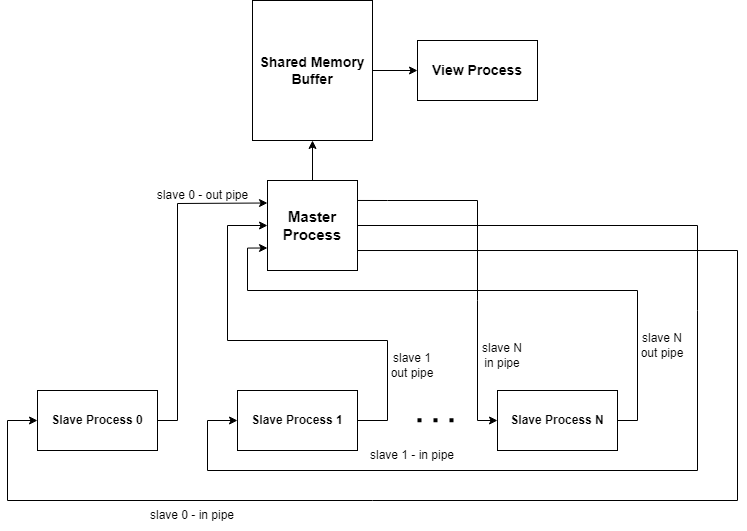
\includegraphics[width=70mm]{diagramaComunicacion}
\caption{Diagrama donde se observa la comunicación entre procesos.}
\label{fig:diagramaComunicacion}
\end{center}
\end{figure}

\section{Compilación y ejecución}

El trabajo práctico fue compilado y ejecutado utilizando la imagen de docker provista por la cátedra. Dentro del contenedor puede ejecutarse los siguientes comandos para compilar el proyecto.

\begin{lstlisting}[language=bash]
$> make clean
$> make
\end{lstlisting}
Una vez compilado, puede ejecutarse el programa principal mediante el siguiente comando.

\begin{lstlisting}[language=bash]
$> ./app file1 file2 ... fileN
\end{lstlisting}
Para también correr el proceso de vista, junto con el programa principal, usando un pipe se puede ejecutar el siguiente comando.
\begin{lstlisting}[language=bash]
$> ./app file1 file2 ... fileN | ./view
\end{lstlisting}
El proceso vista puede ser ejecutado de forma independiente del proceso principal, si el proceso principal está corriendo, se puede ejecutar el proceso vista y ingresar el nombre del semaforo  por teclado (provisto por salida estandar cuando se ejecuta ./app).
\begin{lstlisting}[language=bash]
$> ./view
sem_master
\end{lstlisting}

\section{Limitaciones}

\section{Problemas enfrentados}

\end{document}
